\section{Reordering Vertices for Cache Locality} 
\label{sec:reordering}

\begin{figure}[h]
\centering
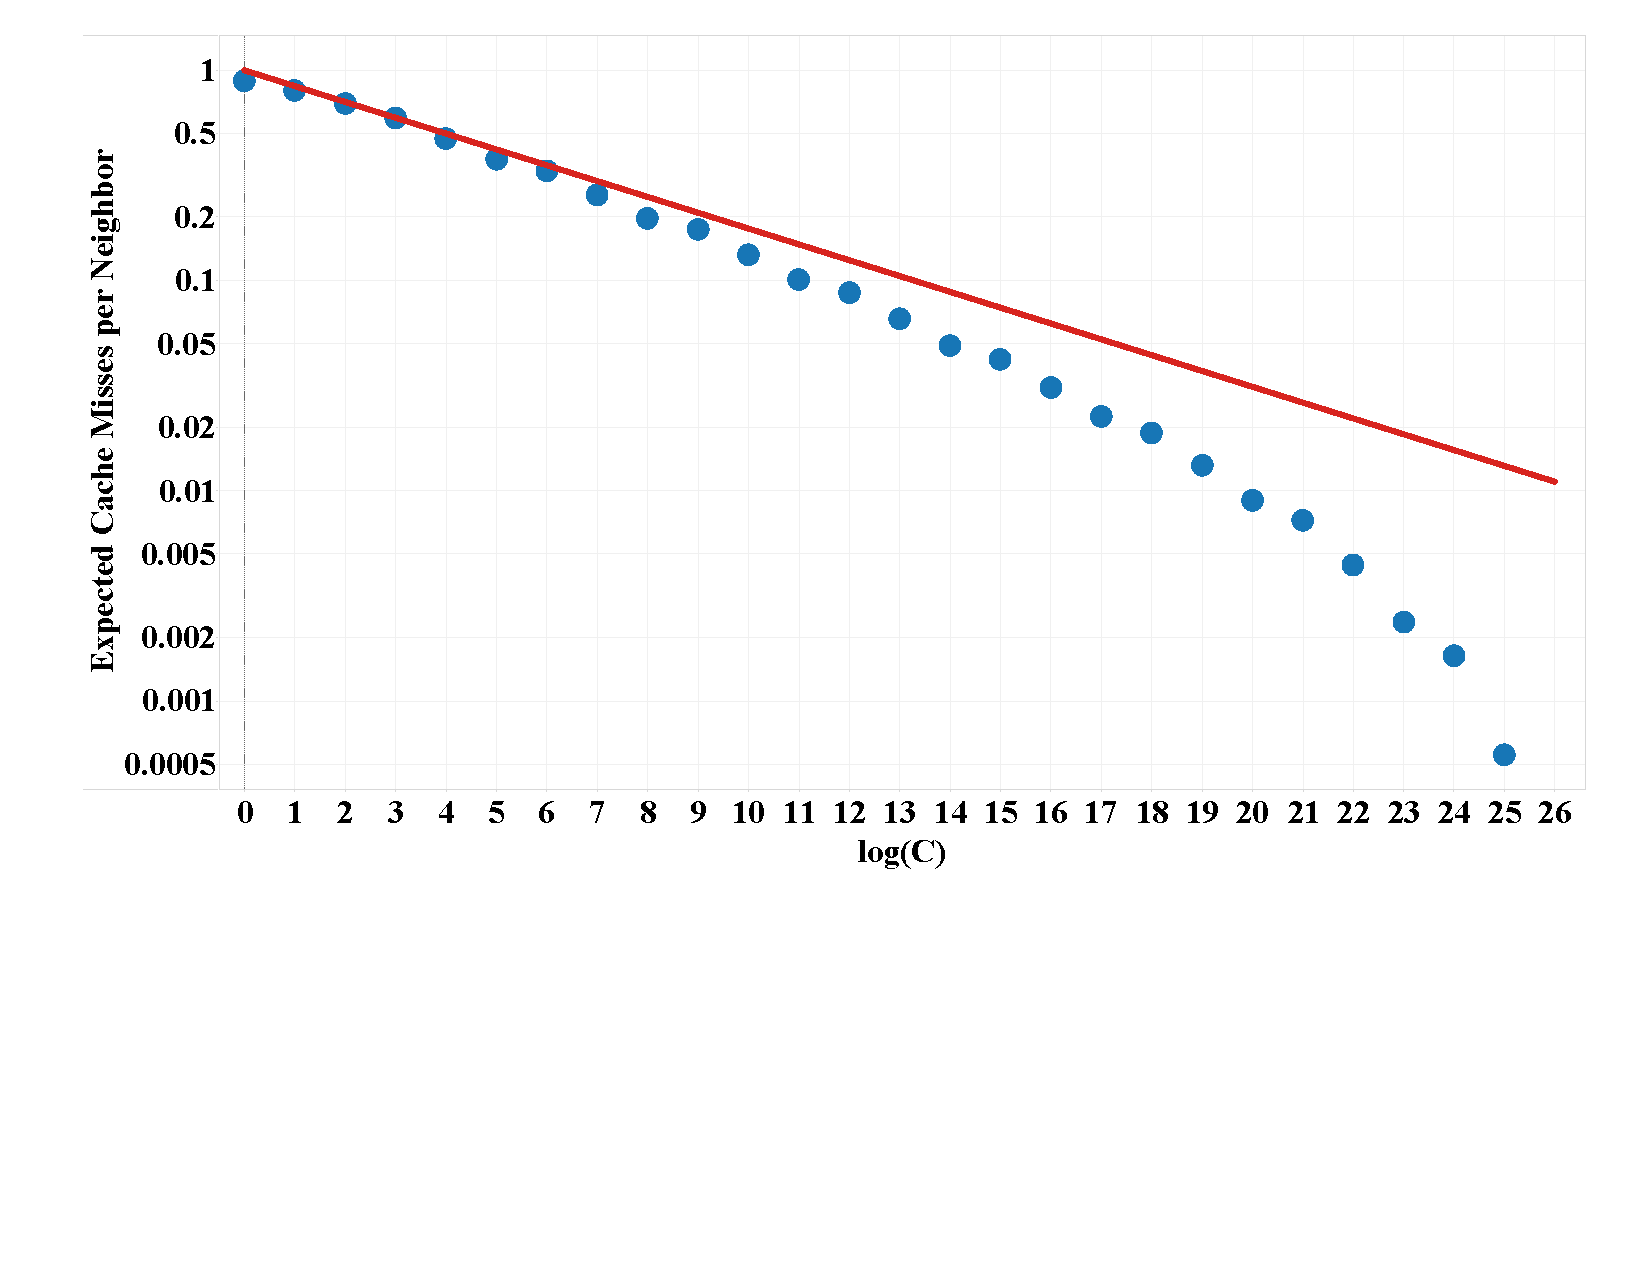
\includegraphics[width=5in,clip,trim=1cm 6cm 0 0]{figures/miss_rate_curve.pdf}
\caption{Theoretical and empirically observed miss rate curves.  The red
line is generated by the equation $C^{-1/4}$, a consequence of the
analysis in Tirthapura et al.~\cite{TirthapuraSeAl06} of generic
recursively-defined space-filling curves.  Hilbert curves are known to
have better locality in practice.  For example, 
the blue dots are empirically measured
from a test graph with 50M vertices described in \secref{empirical}.
}
\label{fig:miss_rate_curve}
\end{figure}

\begin{figure}[h]
\centering
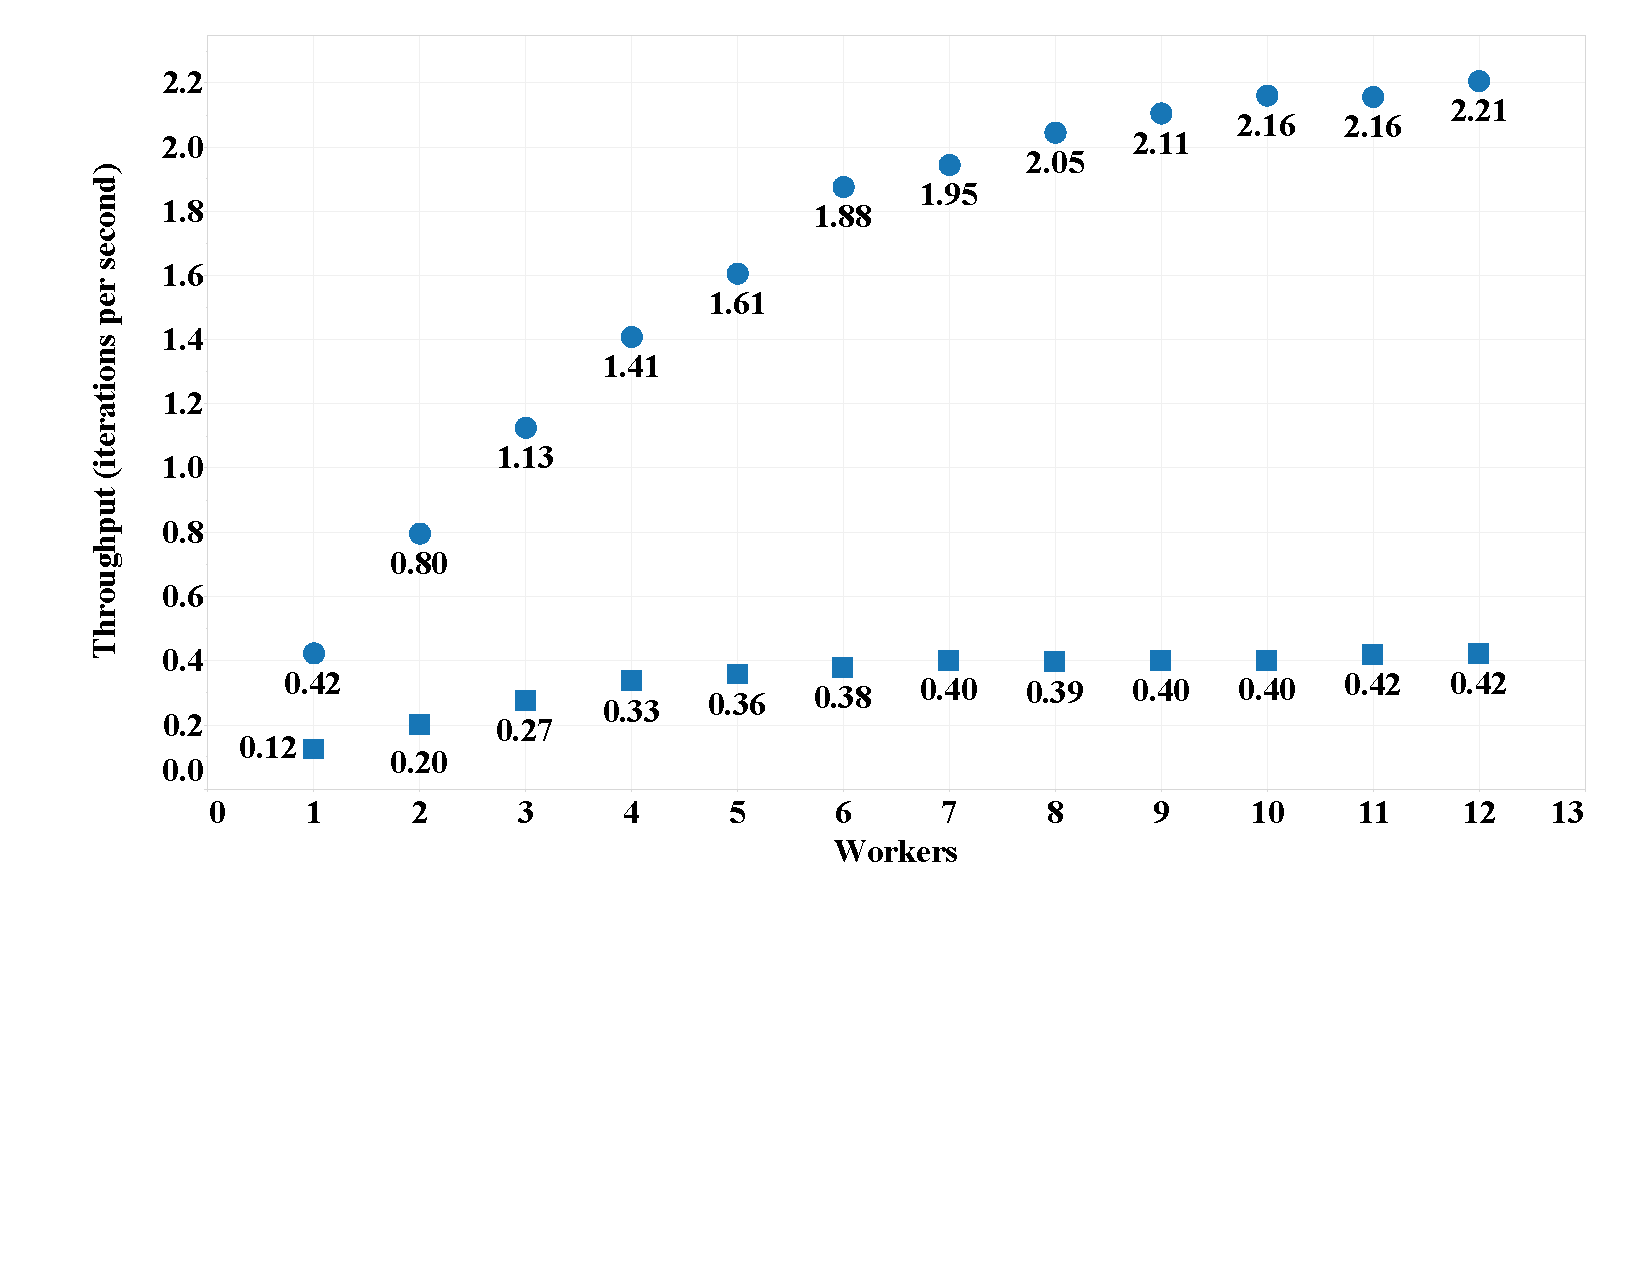
\includegraphics[width=5in,clip,trim=1cm 6cm 0 0]{figures/scalability_bsp.pdf}
\caption{Throughput vs. number of workers of the \proc{BSP} 
scheduling algorithm, described in \figref{bsp_code}, 
for the test graph with 50M vertices described 
in \secref{empirical}.  The squares correspond to the test graph 
with randomly ordered vertices and the circles correspond to the same
graph reordered according to the Hilbert priority function.
}
\label{fig:scalability_bsp}
\end{figure}



\begin{wrapfigure}{r}{.5\textwidth}
\centering
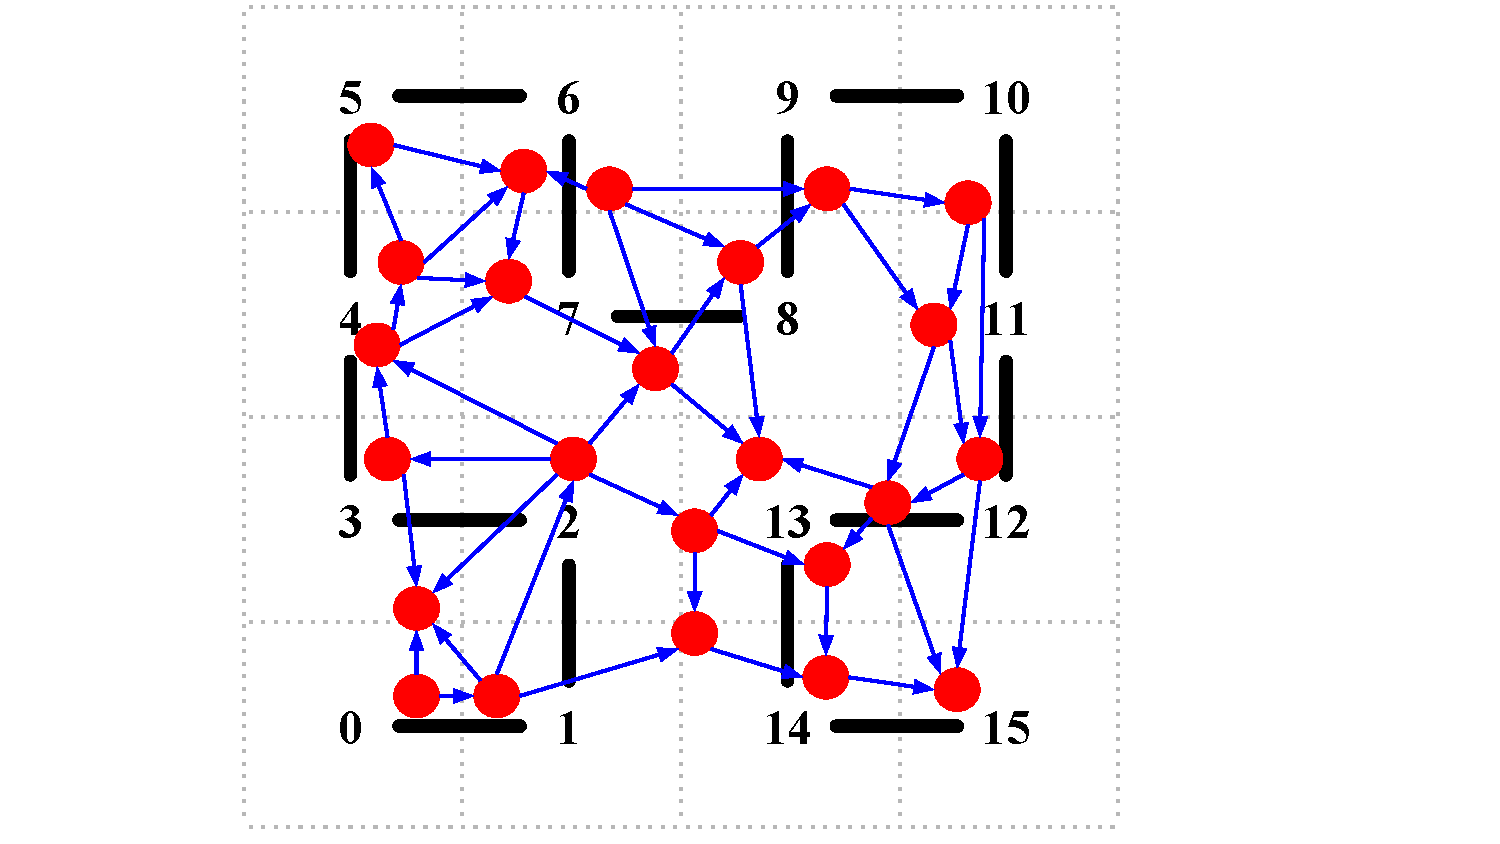
\includegraphics[width=2.5in,clip,trim=4cm 0 4cm 0]{figures/hilbert_priority_function.pdf}
\caption{Example of how a locally-connected graph in 2 dimensions
is mapped to a dag via a second-order Hilbert priority function.  Each
vertex is mapped to its closest grid point in the discretized
Hilbert curve.  Among vertices mapping to the same Hilbert grid
point, ties are broken randomly.}
\label{fig:hilbert_priority}
\end{wrapfigure}


In this section, we will describe the rationale behind and
empirical evidence supporting the use of the
Hilbert space-filling curve as a way of mapping an $N$-dimensional
space onto the real line.  Specifically, we use this mapping
to reorder the vertices of a 3D locally-connected graph to gain cache
locality.  \figref{hilbert_priority} illustrates a set of points
on the unit square overlaid with a second-order 2D Hilbert curve.
The \defn{Hilbert priority function} for a vertex is equal to the value along
the closest Hilbert curve grid point, breaking ties at random.  The
Hilbert priority function takes a parameter $k$ which indicates
the order of the Hilbert curve recursion, where one thinks of the
curve dividing up a cubic space into $2^k$ x $2^k$ x $2^k$ blocks.  This
priority function is used to (comparison) sort the vertices in input graphs
that are known to be locally-connected.\footnote{For problems generated
by Simit, there are generally sufficiently many time steps that any
preprocessing, even $O(n \log n)$-time sorting, are completely 
amortized away.}

We can see in \figref{miss_rate_curve} that reordering the vertices
according to the Hilbert priority function depicted in \figref{hilbert_priority}
yields excellent cache behavior.  For instance, with $\lg (C) = 11$
(i.e. 2048 vertices - roughly the size of the L2 cache in our
Intel Xeon test system) only about 10\% of the neighbors miss the
L2 cache.\footnote{We use the notation $\lg (C)$ to mean $\log_2 (C)$.}



\begin{wrapfigure}{r}{.5\textwidth}
\centering
\begin{codebox*}
	\Procname{$\proc{BSP}(G)$}
	\li 	let $g=(V,E)$
	\li 	\Parfor $v \in V$
	\li 		$\proc{Update}(v)$
		  	\End
\end{codebox*}
\caption{The Bulk-synchronous Parallel (BSP) scheduling algorithm
is the best-case scheduling algorithm in that all vertices are
eligible at the beginning and thus \proc{BSP} incurs the minimum
possible scheduling overhead.}
\label{fig:bsp_code}
\end{wrapfigure}



The red line in \figref{miss_rate_curve}
is the cache miss rate predicted by an analysis in Tirthapura 
et al.~\cite{TirthapuraSeAl06}.  They analyze a generic recursively-defined
space-filling curve, which is pessimistic relative to the Hilbert curve
as we see since our measured miss rates (i.e. the blue circles) 
appear asymptotically lower than the predicted values.
Tirthapura et al. leave as an open problem 
the challenge of analyzing specific space-filling
curves to achieve tighter bounds.  They analyze the problem of 
dividing $n$ vertices uniformly, generated on the unit cube and 
ordered by a space-filling curve, evenly among $n^\alpha$ 
($\alpha \in [0,1]$) processors and 
finding all neighbors for each vertex within a distance $r$, which is
set such that the average degree of the vertices is constant.  They
find that the total number of communications with other processors is
$O(n^{(3+\alpha)/4})$.  Since the average degree is constant there is
$O(n)$ total work and thus the miss rate (i.e. the fraction of neighbors
in another processor's vertex set) is $O(n^{-(1-\alpha)/4})$.  Each
processor is responsible for $n^{1-\alpha}$ vertices.  An immediate
consequence of the result of Tirthapura et al. is that
with a cache of size $C=n^{1-\alpha}$, the expected miss rate
is $O(C^{-1/4})$.  


We use the \proc{BSP} scheduling algorithm, detailed in
\figref{bsp_code}, to demonstrate the 
practical effect of reordering the vertices according to the
Hilbert priority function.  The \proc{BSP} algorithm is quite
simple: merely call \proc{Update} on all vertices in parallel.
The Cilk work-stealing scheduler will tend to give each
worker a contiguous run of vertices to execute and thus exploit
the cache advantage inherent in the vertex reordering.  In 
\figref{scalability_bsp} we see that the throughput achieved by
the input graph reordered by the Hilbert priority function 
(i.e. circles) is much better in absolute terms than the throughput
achieved by the original randomly ordered graph (i.e. squares).

